\documentclass{lab_sheet}
\usepackage[defernumbers=true]{biblatex}
\renewcommand{\lstlistlistingname}{Source Codes}
\renewcommand{\lstlistingname}{Code}
\DeclareBibliographyCategory{cited}
\AtEveryCitekey{\addtocategory{cited}{\thefield{entrykey}}}
\addbibresource{citation.bib}
\nocite{*} 
\begin{document}
\titlePage{Familiarization with 8051/8052 Microcontroller}{September 25, 2020}
\pagenumbering{gobble}
\tableofcontents
\pagebreak
\listoffigures
\pagebreak
\lstlistoflistings
\pagebreak
\pagenumbering{arabic}
\section{Introduction} 
\subsection{Microcontroller}
A microcontroller is an electronic device that consists of all the necessary parts viz. central processing unit, I/O ports, timers, counters, clocks, memory units and registers embedded on a single chip. It is simply a computer capable of performing a specific task and hence are termed as special purpose computers. Generally having small size and low cost, a microcontroller is specifically designed for implementations in embedded systems.
\subsection{MCS-51 Family Microcontroller Chips}
The MCS-51 microcontroller chips, originally developed by Intel for
 use in small-scale embedded systems is based on the Harvard architecture of 
 designing. Initial batches of the chips were designed using the N-type 
 metal-oxide-semiconductors which were later replaced by a more generic MOS, 
 the CMOS (Complementary metal-oxide-semiconductor) hence giving the later 
 versions of the chip the identity of 80C51. Current versions of the microcontroller have clock frequencies of up to 100 MHz, 
which is a drastic improvement from their original 12 MHz clock frequency.\\
The MCS-51 microcontroller was first introduced by Intel in 1980. Since then, 
MCS-51, more commonly termed as the 8051 microcontroller has been adapted by 
various vendors like Silicon Laboratories, ASTX, Dallas Semiconductors, Texas Instruments,
 Atmel and many more for their wide usages in embedded systems.\\\\
The different features of the 8051 microcontroller include:
\begin{itemize}
\item 8-bit ALU, Accumulator and Registers, making it an 8-bit microcontroller.
\item 8-bit data bus meaning that it can access 8 bits of data in one operation.
\item 4KB of ROM for the programs, also called program memory.
\item 128 Bytes of RAM for the variables, also called data memory.
\item 32 I/O lines, i.e. 4 ports with 8 lines each.
\item 16-bit address bus meaning that it can access 65536 locations of RAM and ROM.
\item 2 16-bit timers/counters.
\item 1 full-duplex serial port for serial communication (UART).
\item 6 interrupt sources(2 external interrupts, 2 timer interrupts \& 2 serial interrupts).
\end{itemize}
\subsubsection{Memory Architecture}
The 8051 microcontroller has four different types of memory specifications, viz. Internal RAM, Program Memory, External Data Memory, and Special Function Registers.
\subsubsection*{Internal RAM}
The Internal RAM, or generally referred to as the 
IRAM has an 8-bit address space taking up the addresses from 0x00 to 0xFF. 
IRAM from 0x00 to 0x7F can be accessed directly whereas the remaining must be accessed
 indirectly using the indirect addressing from registers R0 or R1 as @R0 or @R1. 
 The original 8051 microcontroller has 128 bytes of internal RAM whereas some later 
 versions may include 256 bytes of IRAM.
\subsubsection*{Program Memory}
Program memory, referred as PMEM is up to 64 KB of read-only memory, 
starting at address 0 in a separate address space. Both on and off chip versioned
 microcontroller are available in the market.
  PMEM isn't used as much as IRAM and External RAM.\\
  In addition to program code, lookup tables can be stored in the PMEM and 
  retrieved with the MOVC A, @A+DPTR or MOVC A,@A+PC instructions such that 
  the address is calculated with the summation of 8-bit accumulator and 16-bit PC or DPTR.
\subsubsection*{External Data Memory}
XRAM is a third address space memory space starting at address 0 with 16-bit
 address space. It is accessed using the MOVX instruction even though it can 
 be on or off chip.The full 64 KB XRAM can be accessed using MOVX A,@DPTR and MOVX @DPTR,A.
\subsubsection*{Special Function Registers}
SFR are located at the same address as IRAM i.e. at 0x80 to 0xFF and 
accessed just as lower half of IRAM. SFR can only be accessed directly 
since indirect addressing will refer to the remaining half of IRAM. 
SFRs with addresses multiple of 8 are bit-addressable.
\subsubsection{Registers}
Program Counter is the only register in 8051 that isn't memory mapped.
 Eight 8-bit general purpose registers(R0-R7) are mapped to IRAM between 0x00 and 0x1F. 
 Only eight bytes of that range are used at any given time, determined by the two bank select bits in the PSW(RS0 \& RS1). A 8-bit Stack Pointer(SP), 16-bit Data Pointer(DP) and 8-bit Program Status Word(PSW) are also present in the 8051 microcontroller. The PSW doesn't consist of Negative or Zero flags. Parity flag (PSW.0), Overflow(PSW.2), Auxiliary Carry(PSW.6) and Carry(PSW.7) are the other flags of the PSW than the RS0(PSW.3), RS1(PSW.4), User defined(PSW.1) and Flag 0(PSW.5). Accumulator(0xE0) is used by most instructions for storing immediate results and the B register extends the accumulator for multiplication and division routines.
\subsubsection{Programming}
\subsubsection*{Assembly Level Programming}
Pseudo-English representations of the machine languages, or more generally known as Mnemonics are used along side hexadecimal codes to write assembly language codes for the 8051 microcontroller. It is generally written in human understandable mnemonics rather than the actual machine level codes of 0s and 1s. However, it is still a low level programming language and extensive understanding of the architecture is essential. Programs in assembly language are executed faster and occupy less memory. Maximum features of the microcontroller can be used with the help of assembly code and it provides direct and accurate control of all the resources such as I/O ports, RAM, SFRs, etc.
\subsubsection*{High Level Programming}
Various high-level programming languages have different compilers for the MCS-51 family. The most generic of these languages is the embedded C which allows the programmer to specify where variables are stored in the different memory architecture. Since data can be present in one of three memory spaces, IRAM, XRAM and PMEM(read-only), and all these have an address 0, the C compilers have mechanism to determine the memory pointed by either constraining the pointer type to include the memory space, or by storing metadata along with the pointer.\\
Other languages such as C++, Object Pascal, Pascal, BASIC, PL/M, Modula-2 are available for the MCS-51 family but aren't generally in use as compared to the C compilers.
\subsubsection{Instruction Sets}
The instructions in 8051's assembly level programming are all 1 to 3 bytes long. For 3 byte instructions, the first byte represents the operation code, and the last two represent the operands. For most of the instructions, accumulator is necessary but 8051 is not an accumulator based microcontroller. The various mnemonics along with their functions can be looked up in \cite{instruction}.
\section{Objectives}
The primary objective of this lab experiment is to understand the various features and architecture of 8051 microcontroller. Familiarization with the 8051/8052 microcontroller will enable us to write assembly language code for the 8051/8052 microcontroller capable of:
\begin{itemize}
\item Data manipulation
\item Looping and branching techniques
\item Arithmetic and logical operations
\item Subroutine calls
\end{itemize}
\section{Lab Experiment Environment}
The lab experiments will be performed virtually via various simulation softwares. 
The basic usages of these tools allows us to visualize and determine the different 
functional units of the 8051 microcontroller to perform simple arithmetic and logical tasks.
\subsection{Circuit Simulation}
Proteus Design Suite, which is a professional PCB layout, circuit design and simulation tool,
 will be used to simulate the circuit for 8051 microcontroller alongside
  various basic electronic components such as resistors, switches, LEDs, etc. Circuit diagram made in Proteus will consist of a AT89C52 microcontroller with 8-bit LED in a pull-up configuration connected to its Port 0. This circuit will be used to confirm the code written in assembly and C languages.
\subsection{Code Editor and Compiler}
A microcontroller actually only understands hex codes(machine code). 
Writing codes in the machine level language is something that microcontroller 
based companies have tried to avoid. ARM Limited is one such company that produces
 development tools and MDKs along with the hardwares. 
 KEIL products from ARM include C/C++ compilers, debuggers, integrated development and simulation environments, RTOS and middleware libraries, and evaluation boards for ARM, Cortex-M, Cortex-R4, 8051, C166, and 251 processor families. The KEIL $\mu$Vision IDE will be used for writing and assembling the assembly code as well as compiling Embedded C codes into hex code that will be used by the microcontroller. \\
We will be utilizing the compiler from KEIL to generate hex codes and hook that up with the circuit simulation in Proteus for code checking and debugging purpose. KEIL itself provides debugging and simulation features for the 8051 microcontroller, and we will also be using that feature to verify our codes.
\begin{figure}[H]
\centering
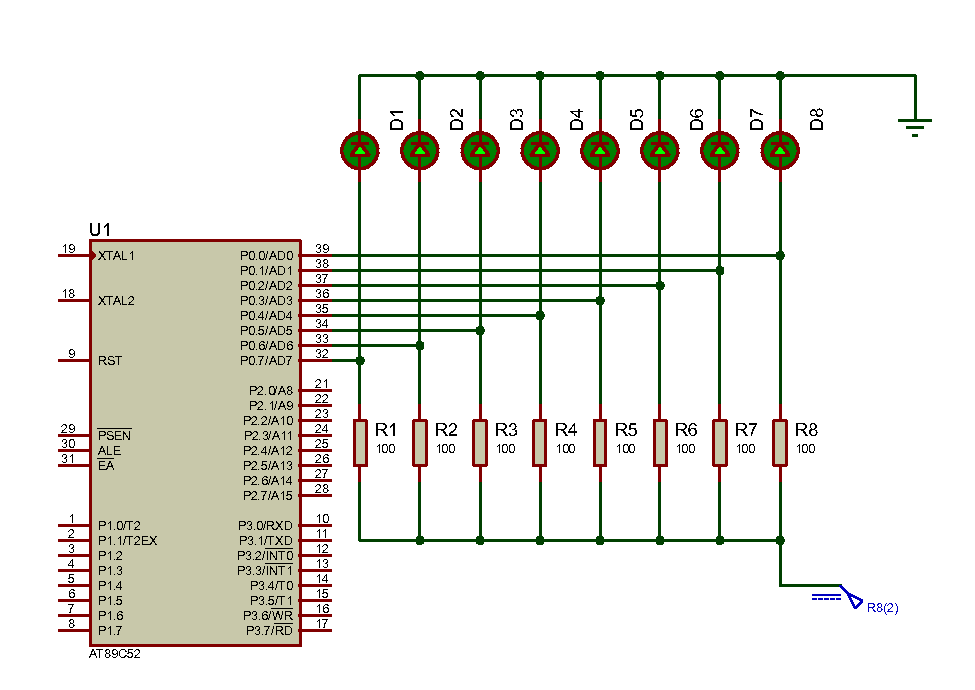
\includegraphics[scale=1]{../Figures/proteus}
\caption{Circuit Diagram for Proteus Simulation}
\label{fig:proteus}
\end{figure}
\section{Lab Problems}
\problem{Write code to add the numbers 897F9AH and 34BC48H and save the result in internal RAM starting at 40H. The result should be displayed continuously on the LEDs of the development board starting from least significant byte with an appropriate timing interval between each byte. Use port zero (P0) of the micro-controller to interface with LEDs.}
\code{lab_1_a}
\problem{Implement a subroutine that replaces the SWAP instruction using rotate right instructions. Test your program on the contents of the accumulator when it contains the number 6BH.}
\code{lab_1_b}
\problem{Multiply, by using looping and successive addition technique, the data in RAM location 22H by the data in RAM location 15H and put the result in RAM locations 19H (low byte) and 1AH (high byte). Data in 22H should be FFH and data in 15H should be DEH.}
\code{lab_1_c}
\problem{Divide, by using looping and successive subtraction technique, the data in RAM location 3EH by the number 12H; put the quotient in R4 and remainder in R5. Data in 3EH should be AFH.}
\code{lab_1_d}
\problem{Store ten hexadecimal numbers in internal RAM starting from memory location 50H. The list of numbers to be used is: D6H, F2H, E4H, A8H, CEH, B9H, FAH, AEH, BAH, CCH. Implement a subroutine that extracts both the smallest and largest numbers from the stored numbers.}
\code{lab_1_e}
\problem{Store ten hexadecimal numbers in internal RAM starting from memory location 60H. The list of numbers to be used is: A5H, FDH, 67H, 42H, DFH, 9AH, 84H, 1BH, C7H, 31H. Implement a subroutine that orders the numbers in ascending order using bubble or any other sort algorithm and implement a subroutine that order the numbers in descending order using selection sort algorithm.}
\subsubsection*{Part I}
\code{lab_1_f1}
\subsubsection*{Part II}
\code{lab_1_f2}
\problem{Store numbers from 00H to 20H in internal RAM starting from memory location 40H. Implement a subroutine that extracts only the prime numbers.}
\code{lab_1_g}
\problem{Find the factorial of a number stored in R3. The value in R3 could be any number in the range from 00H to 05H. Implement a subroutine that calculates the factorial. The factorial needs to be represented in both hexadecimal and decimal formats.}
\code{lab_1_h}
\section{Observations}
The observations for all the lab problems are presented in this section. Port 0 display values are snipped from KEIL $\mu$Vision IDE in debug mode with appropriate breakpoints. The internal RAM and register values are snipped from the Proteus simulation during the VSM debugging. These values simulate the hardware for 8051 MCU so slight variation from the actual states may be visible. Since the lab experiments are performed in simulated environment, the following observations are chosen such that higher accuracy in data visualization for 8051 registers, ports and IRAM can be made. Circuit behaviors from Proteus simulation aren't included in this report, however the observations are clear enough to make conclusions for the lab.
\subsection*{Problem 1}
\begin{figure}[H]
\begin{subfigure}{.5\textwidth}
  \centering
  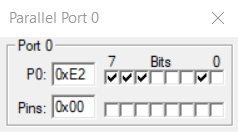
\includegraphics[frame,width=.8\linewidth]{../Figures/1_1_a.png}  
  \label{fig:prob1-a}
  \caption{}
\end{subfigure}
\begin{subfigure}{.5\textwidth}
  \centering
  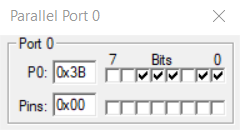
\includegraphics[frame,width=.8\linewidth]{../Figures/1_1_b.png}  
  \label{fig:prob1-b}
  \caption{}
\end{subfigure}
\newline
\begin{subfigure}{.5\textwidth}
  \centering
    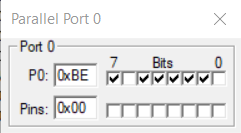
\includegraphics[frame,width=.8\linewidth]{../Figures/1_1_c.png}  
  \label{fig:prob1-c}
  \caption{}
\end{subfigure}
\begin{subfigure}{.5\textwidth}
  \centering
  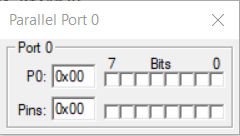
\includegraphics[frame,width=.8\linewidth]{../Figures/1_1_d.png}   
  \caption{}
  \label{fig:prob1-d}
\end{subfigure}
\newline
\hspace*{\fill}
\begin{subfigure}{.5\textwidth}
  \centering
  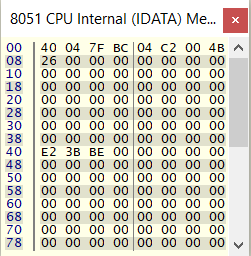
\includegraphics[frame,width=.8\linewidth]{../Figures/1_1_e.png}   
  \caption{}
  \label{fig:prob1-e}
\end{subfigure}
\hspace*{\fill}
\caption{Observations for Problem 1}
\label{fig:prob1}
\end{figure}
Figure(\ref{fig:prob1}) shows the various outputs on Port 0 during the execution of Problem 1. The addition of 897F9AH and 34BC48H gives 00BE3BE2H which is continuously displayed on Port 0 starting from the LSB. Moreover, Figure(\ref{fig:prob1-e}) shows the IRAM values once the program is run on Proteus simulation. The result for the addition is stored starting from the LSB at 40H location. 
\subsection*{Problem 2}
\begin{figure}[H]
\begin{subfigure}{.5\textwidth}
  \centering
  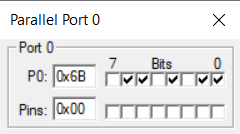
\includegraphics[frame,width=.8\linewidth]{../Figures/1_2_a.png}  
  \label{fig:prob2-a}
  \caption{}
\end{subfigure}
\begin{subfigure}{.5\textwidth}
  \centering
  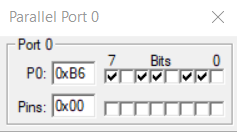
\includegraphics[frame,width=.8\linewidth]{../Figures/1_2_b.png}  
  \label{fig:prob2-b}
  \caption{}
\end{subfigure}
\caption{Observations for Problem 2}
\label{fig:prob2}
\end{figure}
Figure(\ref{fig:prob2}) shows the output on Port 0 on execution of Problem 2. The upper and lower nibbles of accumulator are swapped without using the SWAP instruction. Hence, 6BH becomes B6H once the swap is performed.
\subsection*{Problem 3}
\begin{figure}[H]
\begin{subfigure}{.5\textwidth}
  \centering
  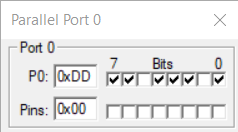
\includegraphics[frame,width=.8\linewidth]{../Figures/1_3_a.png}  
  \label{fig:prob3-a}
  \caption{}
\end{subfigure}
\begin{subfigure}{.5\textwidth}
  \centering
  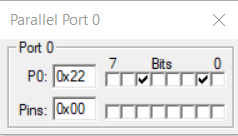
\includegraphics[frame,width=.8\linewidth]{../Figures/1_3_b.png}  
  \label{fig:prob3-b}
  \caption{}
\end{subfigure}
\newline
\hspace*{\fill}
\begin{subfigure}{.5\textwidth}
  \centering
  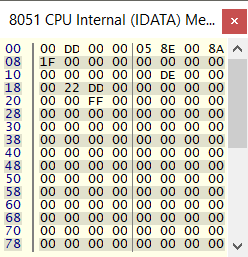
\includegraphics[frame,width=.8\linewidth]{../Figures/1_3_c.png}   
  \caption{}
  \label{fig:prob3-c}
\end{subfigure}
\hspace*{\fill}
\caption{Observations for Problem 3}
\label{fig:prob3}
\end{figure}
Figure(\ref{fig:prob3}) shows the result of multiplication of FFH and DEH i.e. DD22H in Port 0. Moreover, the low byte is stored in IRAM location 19H and high byte in 1AH as required by the question which is clear from Figure(\ref{fig:prob3-c}).
\subsection*{Problem 4}
\begin{figure}[H]
\begin{subfigure}{.5\textwidth}
  \centering
  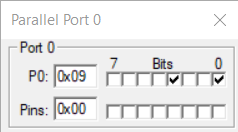
\includegraphics[frame,width=.8\linewidth]{../Figures/1_4_a.png}  
  \label{fig:prob4-a}
  \caption{}
\end{subfigure}
\begin{subfigure}{.5\textwidth}
  \centering
  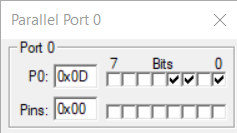
\includegraphics[frame,width=.8\linewidth]{../Figures/1_4_b.png}  
  \label{fig:prob4-b}
  \caption{}
\end{subfigure}
\newline
\hspace*{\fill}
\begin{subfigure}{.5\textwidth}
  \centering
  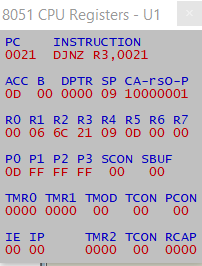
\includegraphics[frame,width=.8\linewidth]{../Figures/1_4_c.png}   
  \caption{}
  \label{fig:prob4-c}
\end{subfigure}
\hspace*{\fill}
\caption{Observations for Problem 4}
\label{fig:prob4}
\end{figure}
Figure(\ref{fig:prob4}) displays the output for division of AFH by 12H, i.e. quotient=09H and remainder=0DH on the Port 0. The values of quotient and remainder are also stored in R4 and R5 registers as required by the question, which is visible from Figure(\ref{fig:prob4-c}).
\subsection*{Problem 5}
\begin{figure}[H]
\hspace*{\fill}
\begin{subfigure}{.5\textwidth}
  \centering
  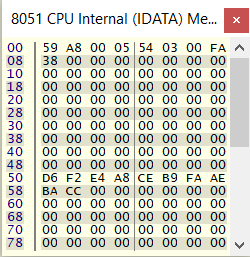
\includegraphics[frame,width=.8\linewidth]{../Figures/1_5_a.png}   
  \caption{}
  \label{fig:prob5-a}
\end{subfigure}
\hspace*{\fill}
\newline
\begin{subfigure}{.5\textwidth}
  \centering
  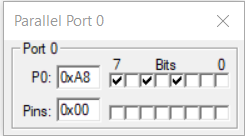
\includegraphics[frame,width=.8\linewidth]{../Figures/1_5_b.png}  
  \label{fig:prob5-b}
  \caption{}
\end{subfigure}
\begin{subfigure}{.5\textwidth}
  \centering
  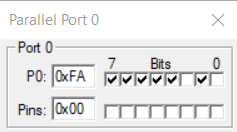
\includegraphics[frame,width=.8\linewidth]{../Figures/1_5_c.png}  
  \label{fig:prob5-c}
  \caption{}
\end{subfigure}
\caption{Observations for Problem 5}
\label{fig:prob5}
\end{figure}
Figure(\ref{fig:prob5}) shows the display on Port 0 for the smallest and largest hexadecimal numbers i.e. A8H and FAH from a list of 10 numbers stored in the IRAM location starting from 50H, which is observed in Figure(\ref{fig:prob5-a}).
\subsection*{Problem 6}
\begin{figure}[H]
\begin{subfigure}{.5\textwidth}
  \centering
  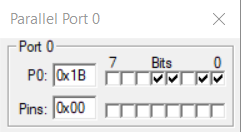
\includegraphics[frame,width=.8\linewidth]{../Figures/1_6_a.png}  
  \caption{}
   \label{fig:prob6a-a}
\end{subfigure}
\begin{subfigure}{.5\textwidth}
  \centering
  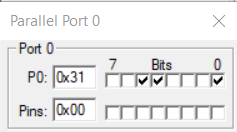
\includegraphics[frame,width=.8\linewidth]{../Figures/1_6_b.png}  
  \caption{}
  \label{fig:prob6a-b}
\end{subfigure}
\caption{Observations for Problem 6 - Part I}
\label{fig:prob6a}
\end{figure}
\begin{figure}[H]\ContinuedFloat
\begin{subfigure}{.5\textwidth}
  \centering
    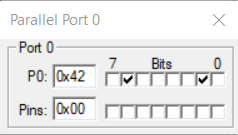
\includegraphics[frame,width=.8\linewidth]{../Figures/1_6_c.png}  
  \label{fig:prob6a-c}
  \caption{}
\end{subfigure}
\begin{subfigure}{.5\textwidth}
  \centering
  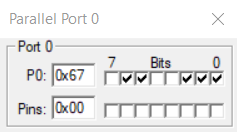
\includegraphics[frame,width=.8\linewidth]{../Figures/1_6_d.png}   
  \caption{}
  \label{fig:prob6a-d}
\end{subfigure}
\begin{subfigure}{.5\textwidth}
  \centering
  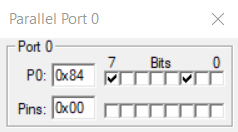
\includegraphics[frame,width=.8\linewidth]{../Figures/1_6_e.png}  
  \label{fig:prob6a-e}
  \caption{}
\end{subfigure}
\begin{subfigure}{.5\textwidth}
  \centering
  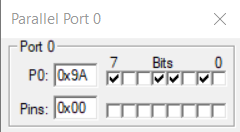
\includegraphics[frame,width=.8\linewidth]{../Figures/1_6_f.png}  
  \label{fig:prob6a-f}
  \caption{}
\end{subfigure}
\begin{subfigure}{.5\textwidth}
  \centering
    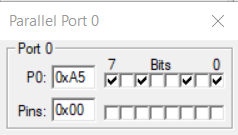
\includegraphics[frame,width=.8\linewidth]{../Figures/1_6_g.png}  
  \label{fig:prob6a-g}
  \caption{}
\end{subfigure}
\begin{subfigure}{.5\textwidth}
  \centering
  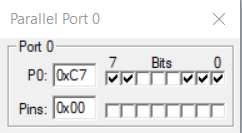
\includegraphics[frame,width=.8\linewidth]{../Figures/1_6_h.png}   
  \caption{}
  \label{fig:prob6a-h}
\end{subfigure}
\begin{subfigure}{.5\textwidth}
  \centering
  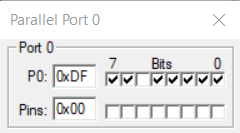
\includegraphics[frame,width=.8\linewidth]{../Figures/1_6_i.png}   
  \caption{}
  \label{fig:prob6a-i}
\end{subfigure}
\begin{subfigure}{.5\textwidth}
  \centering
  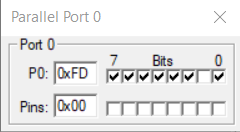
\includegraphics[frame,width=.8\linewidth]{../Figures/1_6_j.png}   
  \caption{}
  \label{fig:prob6a-j}
\end{subfigure}
\caption*{Figure~\ref{fig:prob6a}:~Observations for Problem 6 - Part I (continued)}
\end{figure}
Figure(\ref{fig:prob6a}) shows the different Port 0 outputs which are actually the 10 hexadecimal numbers sorted in ascending order using bubble sort algorithm. Port 0 observations from Figure(\ref{fig:prob6a-a}) to Figure(\ref{fig:prob6a-j}) are arranged in ascending order. 
\begin{figure}[H]
\begin{subfigure}{.5\textwidth}
  \centering
  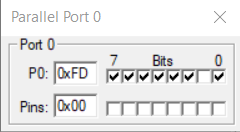
\includegraphics[frame,width=.8\linewidth]{../Figures/1_6_j.png}  
  \caption{}
  \label{fig:prob6b-a}
\end{subfigure}
\begin{subfigure}{.5\textwidth}
  \centering
  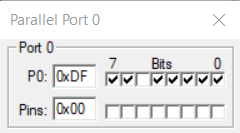
\includegraphics[frame,width=.8\linewidth]{../Figures/1_6_i.png}  
  \label{fig:prob6b-b}
  \caption{}
\end{subfigure}
\begin{subfigure}{.5\textwidth}
  \centering
    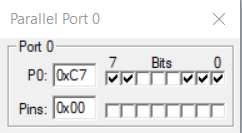
\includegraphics[frame,width=.8\linewidth]{../Figures/1_6_h.png}  
  \label{fig:prob6b-c}
  \caption{}
\end{subfigure}
\begin{subfigure}{.5\textwidth}
  \centering
  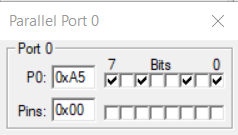
\includegraphics[frame,width=.8\linewidth]{../Figures/1_6_g.png}   
  \caption{}
  \label{fig:prob6b-d}
\end{subfigure}
\begin{subfigure}{.5\textwidth}
  \centering
  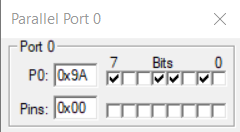
\includegraphics[frame,width=.8\linewidth]{../Figures/1_6_f.png}  
  \label{fig:prob6b-e}
  \caption{}
\end{subfigure}
\begin{subfigure}{.5\textwidth}
  \centering
  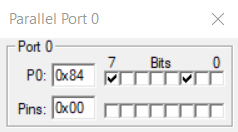
\includegraphics[frame,width=.8\linewidth]{../Figures/1_6_e.png}  
  \label{fig:prob6b-f}
  \caption{}
\end{subfigure}
\begin{subfigure}{.5\textwidth}
  \centering
    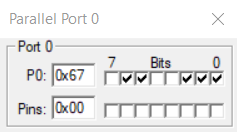
\includegraphics[frame,width=.8\linewidth]{../Figures/1_6_d.png}  
  \label{fig:prob6b-g}
  \caption{}
\end{subfigure}
\begin{subfigure}{.5\textwidth}
  \centering
  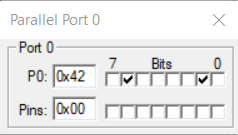
\includegraphics[frame,width=.8\linewidth]{../Figures/1_6_c.png}   
  \caption{}
  \label{fig:prob6b-h}
\end{subfigure}
\begin{subfigure}{.5\textwidth}
  \centering
    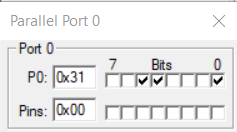
\includegraphics[frame,width=.8\linewidth]{../Figures/1_6_b.png}  
  \label{fig:prob6b-i}
  \caption{}
\end{subfigure}
\begin{subfigure}{.5\textwidth}
  \centering
  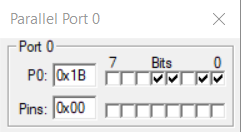
\includegraphics[frame,width=.8\linewidth]{../Figures/1_6_a.png}   
  \caption{}
  \label{fig:prob6b-j}
\end{subfigure}
\caption{Observations for Problem 6 - Part II}
\label{fig:prob6b}
\end{figure}
Figure(\ref{fig:prob6b}) shows the different Port 0 outputs which are actually the 10 hexadecimal numbers sorted in descending order using selection sort algorithm. Port 0 observations from Figure(\ref{fig:prob6b-a}) to Figure(\ref{fig:prob6b-j}) are arranged in descending order.
\begin{figure}[H]
\begin{subfigure}{.5\textwidth}
  \centering
  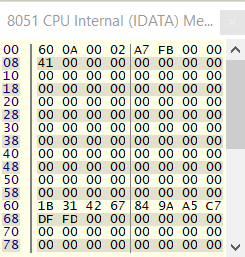
\includegraphics[frame,width=.8\linewidth]{../Figures/1_6_k.png}  
    \caption{}
  \label{fig:prob6-asc}
\end{subfigure}
\begin{subfigure}{.5\textwidth}
  \centering
  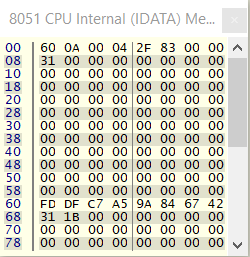
\includegraphics[frame,width=.8\linewidth]{../Figures/1_6_l.png}  
    \caption{}
  \label{fig:prob6-dec}
\end{subfigure}
\caption{IRAM observations for Problem 6}
\label{fig:prob6-IRAM}
\end{figure}
Figure(\ref{fig:prob6-asc}) shows the IRAM values for Problem 6 - Part I where the hexadecimal numbers from 60H are sorted in ascending order. Likewise, Figure(\ref{fig:prob6-dec}) shows the Problem 6 - Part II observations where the same hexadecimal numbers are arranged in descending order.
\subsection*{Problem 7}
Figure(\ref{fig:prob7}) shows the Port 0 outputs for the Problem 7 where only the prime numbers among 00H to 20H stored in memory location starting from 40H were to be shown. Figure(\ref{fig:prob7-a}) to Figure(\ref{fig:prob7-k}) display the prime numbers in that range.
\begin{figure}[H]
\begin{subfigure}{.5\textwidth}
  \centering
  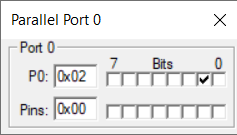
\includegraphics[frame,width=.8\linewidth]{../Figures/1_7_a.png}  
  \caption{}
   \label{fig:prob7-a}
\end{subfigure}
\begin{subfigure}{.5\textwidth}
  \centering
  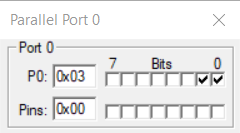
\includegraphics[frame,width=.8\linewidth]{../Figures/1_7_b.png}  
  \caption{}
  \label{fig:prob7-b}
\end{subfigure}
\caption{Observations for Problem 7}
\label{fig:prob7}
\end{figure}
\begin{figure}[H]\ContinuedFloat
\begin{subfigure}{.5\textwidth}
  \centering
    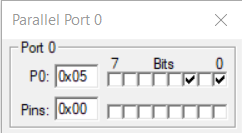
\includegraphics[frame,width=.8\linewidth]{../Figures/1_7_c.png}  
  \label{fig:prob7-c}
  \caption{}
\end{subfigure}
\begin{subfigure}{.5\textwidth}
  \centering
  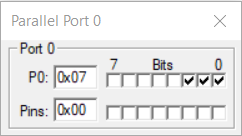
\includegraphics[frame,width=.8\linewidth]{../Figures/1_7_d.png}   
  \caption{}
  \label{fig:prob7-d}
\end{subfigure}
\begin{subfigure}{.5\textwidth}
  \centering
  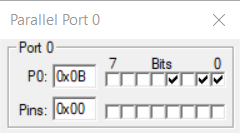
\includegraphics[frame,width=.8\linewidth]{../Figures/1_7_e.png}  
  \label{fig:prob7-e}
  \caption{}
\end{subfigure}
\begin{subfigure}{.5\textwidth}
  \centering
  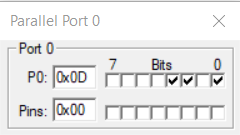
\includegraphics[frame,width=.8\linewidth]{../Figures/1_7_f.png}  
  \label{fig:prob7-f}
  \caption{}
\end{subfigure}
\begin{subfigure}{.5\textwidth}
  \centering
    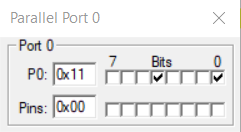
\includegraphics[frame,width=.8\linewidth]{../Figures/1_7_g.png}  
  \label{fig:prob7-g}
  \caption{}
\end{subfigure}
\begin{subfigure}{.5\textwidth}
  \centering
  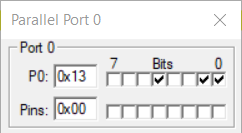
\includegraphics[frame,width=.8\linewidth]{../Figures/1_7_h.png}   
  \caption{}
  \label{fig:prob7-h}
\end{subfigure}
\begin{subfigure}{.5\textwidth}
  \centering
  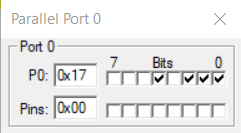
\includegraphics[frame,width=.8\linewidth]{../Figures/1_7_i.png}   
  \caption{}
  \label{fig:prob7-i}
\end{subfigure}
\begin{subfigure}{.5\textwidth}
  \centering
  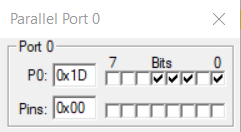
\includegraphics[frame,width=.8\linewidth]{../Figures/1_7_j.png}   
  \caption{}
  \label{fig:prob7-j}
\end{subfigure}
\hspace*{\fill}
\begin{subfigure}{.5\textwidth}
  \centering
  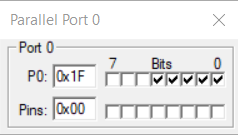
\includegraphics[frame,width=.8\linewidth]{../Figures/1_7_k.png}   
  \caption{}
  \label{fig:prob7-k}
\end{subfigure}
\hspace*{\fill}
\caption*{Figure~\ref{fig:prob7}:~Observations for Problem 7 (continued)}
\end{figure}
\subsection*{Problem 8}
\begin{figure}[H]
\begin{subfigure}{.5\textwidth}
  \centering
  \includegraphics[frame,width=.8\linewidth]{../Figures/1_8_a.png}   
  \caption{}
  \label{fig:prob8-a}
\end{subfigure}
\begin{subfigure}{.5\textwidth}
  \centering
  \includegraphics[frame,width=.8\linewidth]{../Figures/1_8_b.png}   
  \caption{}
  \label{fig:prob8-b}
\end{subfigure}
\begin{subfigure}{.5\textwidth}
  \centering
  \includegraphics[frame,width=.8\linewidth]{../Figures/1_8_c.png}   
  \caption{}
  \label{fig:prob8-c}
\end{subfigure}
\begin{subfigure}{.5\textwidth}
  \centering
  \includegraphics[frame,width=.8\linewidth]{../Figures/1_8_d.png}   
  \caption{}
  \label{fig:prob8-d}
\end{subfigure}
\caption{Observations for Problem 8 - Embedded C}
\label{fig:prob8}
\end{figure}
The hexadecimal number under observation in R3 is 04H. So the factorial of 04H is 18H which is shown in Figure(\ref{fig:prob8-a}). The decimal equivalent of this is shown in three digits i.e. units, tens and hundreds place in Figure(\ref{fig:prob8-b}), Figure(\ref{fig:prob8-c}) and Figure(\ref{fig:prob8-d}) respectively. The observation for the assembly level code was slightly different for this problem.
\begin{figure}[H]
\begin{subfigure}{.5\textwidth}
  \centering
  \includegraphics[frame,width=.8\linewidth]{../Figures/1_8_a.png}   
  \caption{}
  \label{fig:prob9-a}
\end{subfigure}
\begin{subfigure}{.5\textwidth}
  \centering
  \includegraphics[frame,width=.8\linewidth]{../Figures/1_8_e.png}   
  \caption{}
  \label{fig:prob9-b}
\end{subfigure}
\hspace*{\fill}
\begin{subfigure}{.5\textwidth}
  \centering
  \includegraphics[frame,width=.8\linewidth]{../Figures/1_8_d.png}   
  \caption{}
  \label{fig:prob9-c}
\end{subfigure}
\hspace*{\fill}
\caption{Observations for Problem 8 - Assembly}
\label{fig:prob9}
\end{figure}
\section{Discussion}
In this lab experiment, the 8051/52 microcontroller programming was dealt 
with various levels of problems. Addition, subtraction, 
rotation, multiplication, division, additional data manipulation, 
various logical operations based on flags and subroutine calls were 
included in the problems that allowed us to be familiar with the basic
 programming approaches to 8051/52 MCUs.
  Moreover, the use of KEIL $\mu$Vision IDE along with Proteus for circuit simulation 
  allowed us to realize the problems in a practical approach. This lab allowed us to 
  learn the basics of programming a 8051/52 MCU in KEIL using both assembly level and
   Embedded C language. The hex codes generated were then burnt into the simulated circuit 
   in Proteus shown in Figure(\ref{fig:proteus}) to visualize the results. 
   The port values, IRAM data and register values were visualized from both 
   KEIL $\mu$Vision and Proteus in debugging modes such that they represent 
   the output of the problems.
\printbibliography[heading=bibintoc,title={Bibliography}, category=cited]
\printbibliography[heading=bibintoc,title={Additional References},notcategory=cited]
\end{document} 